\chapter{Oxydation et réduction}\label{ch:g11:redox}

On plonge une lame de zinc dans une solution bleue de sulfate de cuivre.
En quelques minutes, sa surface se couvre d'un dépôt spongieux brun-rouge~;
une heure plus tard, le bleu de la solution a pâli. Du cuivre métallique
est apparu là où il n'y en avait pas, et le zinc est passé en solution
sous forme d'\omterm{def:g9:ions:ion}{ions} invisibles. Rien n'a été chauffé, aucun gaz ne s'est
dégagé, aucun dioxygène n'est intervenu --- et pourtant les chimistes
appellent cela une \omterm{def:g11:redox:oxidation}{oxydation}. Le mot voulait autrefois dire «~combinaison
avec l'oxygène~»~; il désigne aujourd'hui quelque chose de plus général
et de plus utile~: la perte d'\omterm{def:g9:inside-the-atom:nucleus}{électrons}. Ce chapitre suit les \omterm{def:g9:inside-the-atom:nucleus}{électrons}.

\begin{recall}
Un \omterm{def:g9:ions:ion}{ion} est un \omterm{def:g7:atoms-and-molecules:atom}{atome} ou un groupe d'\omterm{def:g7:atoms-and-molecules:atom}{atomes} qui a gagné ou perdu des
\omterm{def:g9:inside-the-atom:nucleus}{électrons} (\cref{ch:g9:ions}). Un \omterm{def:g9:periodic-table-first-look:metal}{métal} comme le fer ou le zinc réagit
avec l'acide chlorhydrique en donnant du dihydrogène et des \omterm{def:g9:ions:ion}{ions}
métalliques (\cref{ch:g9:metals-acids-corrosion}). Une \omterm{def:g10:the-mole:amount}{quantité de
matière} $n$, en \omterm{def:g10:the-mole:amount}{moles}, se calcule à partir d'une masse $m$ par
$n = m/M$ (\cref{ch:g10:the-mole}).
\end{recall}

\begin{omfigure}
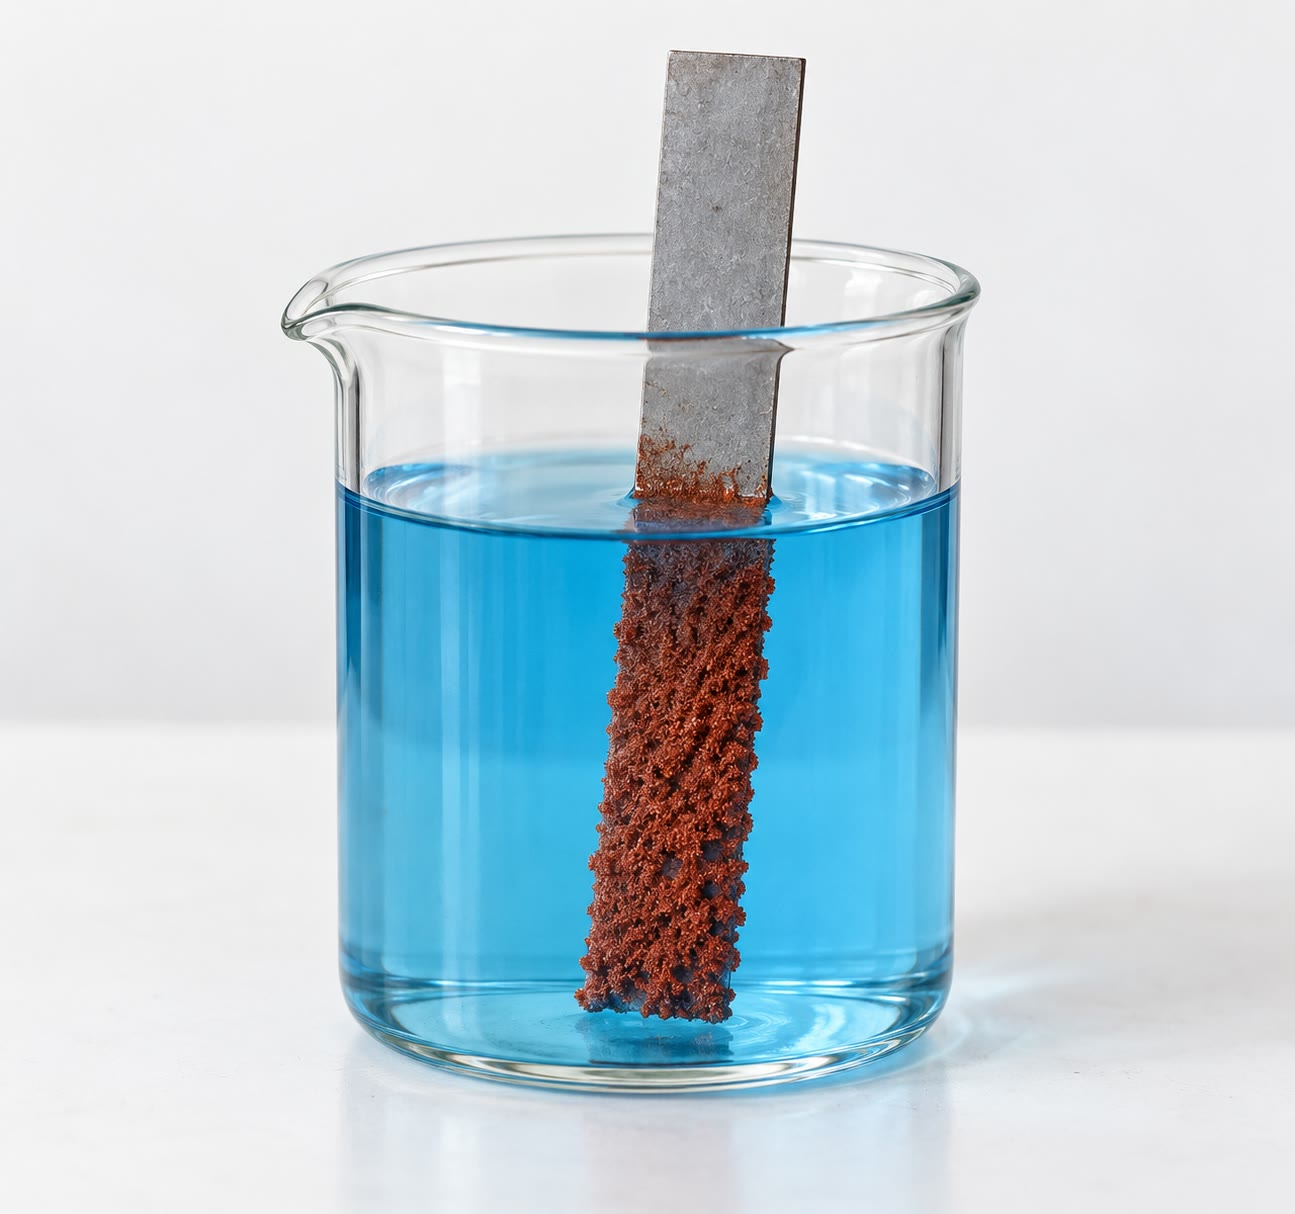
\includegraphics[width=0.55\linewidth]{images/book1/ai/g11-zinc-copper-sulfate.jpg}

{\small Une lame de zinc dans une solution de sulfate de cuivre~: du
cuivre se dépose sur le zinc, et des \omterm{def:g9:ions:ion}{ions} zinc prennent sa place dans la
solution.}
\end{omfigure}

\section{Oxydants et réducteurs}

\begin{definition}[Oxydant et réducteur]\label{def:g11:redox:oxidant}
Un \emph{oxydant}\index{oxydant} est une espèce capable de gagner un ou
plusieurs \omterm{def:g9:inside-the-atom:nucleus}{électrons}. Un \emph{réducteur}\index{reducteur@réducteur} est une espèce
capable de céder un ou plusieurs \omterm{def:g9:inside-the-atom:nucleus}{électrons}.
\end{definition}

\begin{definition}[Oxydation et réduction]\label{def:g11:redox:oxidation}
Une \emph{oxydation}\index{oxydation} est une perte d'\omterm{def:g9:inside-the-atom:nucleus}{électrons}~; une
\emph{réduction}\index{reduction@réduction} est un gain d'\omterm{def:g9:inside-the-atom:nucleus}{électrons}. Un \omterm{def:g11:redox:oxidant}{réducteur}
s'oxyde~; un \omterm{def:g11:redox:oxidant}{oxydant} se réduit.
\end{definition}

\begin{remark}[Un moyen mnémotechnique]\label{rem:g11:redox:remember}
Lors d'une \emph{\omterm{def:g11:redox:oxidation}{réduction}}, la charge de l'espèce est réduite~:
\ce{Cu^{2+}} qui gagne deux \omterm{def:g9:inside-the-atom:nucleus}{électrons} devient \ce{Cu}, charge $+2 \to 0$.
Lors d'une \omterm{def:g11:redox:oxidation}{oxydation}, la charge augmente~: \ce{Zn -> Zn^{2+} + 2e-},
$0 \to +2$.
\end{remark}

\begin{definition}[Couple oxydant/réducteur et demi-équation]\label{def:g11:redox:couple}
Un \omterm{def:g11:redox:oxidant}{oxydant} et le \omterm{def:g11:redox:oxidant}{réducteur} qu'il devient en gagnant des \omterm{def:g9:inside-the-atom:nucleus}{électrons} forment
un \emph{couple oxydant/réducteur}\index{couple oxydant/reducteur@couple oxydant/réducteur}, noté
Ox/Red, l'\omterm{def:g11:redox:oxidant}{oxydant} en premier~: \ce{Cu^{2+}}/\ce{Cu},
\ce{Zn^{2+}}/\ce{Zn}. L'échange d'\omterm{def:g9:inside-the-atom:nucleus}{électrons} au sein d'un couple est
décrit par sa \emph{demi-équation}\index{demi-equation@demi-équation},
\[
  \text{Ox} + n\,\ce{e-} \ce{<=>} \text{Red}, % ce-unbalanced-ok (generic form)
\]
ajustée en \omterm{def:g7:atoms-and-molecules:atom}{atomes} et en charges, par exemple
$\ce{Cu^{2+}(aq) + 2e- <=> Cu(s)}$. La double flèche indique que
l'échange peut se faire dans les deux sens.
\end{definition}

\begin{example}[Les métaux et leurs ions]\label{ex:g11:redox:metals}
Chaque \omterm{def:g9:periodic-table-first-look:metal}{métal} forme un couple avec son \omterm{def:g9:ions:ion}{ion}~:
\begin{center}
\begin{tabular}{ll}
\hline
couple & \omterm{def:g11:redox:couple}{demi-équation} \\
\hline
\ce{Ag+}/\ce{Ag} & \ce{Ag+ + e- <=> Ag} \\
\ce{Cu^{2+}}/\ce{Cu} & \ce{Cu^{2+} + 2e- <=> Cu} \\
\ce{Fe^{2+}}/\ce{Fe} & \ce{Fe^{2+} + 2e- <=> Fe} \\
\ce{Zn^{2+}}/\ce{Zn} & \ce{Zn^{2+} + 2e- <=> Zn} \\
\ce{Al^{3+}}/\ce{Al} & \ce{Al^{3+} + 3e- <=> Al} \\
\hline
\end{tabular}
\end{center}
Des \omterm{def:g9:ions:ion}{ions} peuvent aussi former des couples~: \ce{Fe^{3+} + e- <=> Fe^{2+}}
pour le couple \ce{Fe^{3+}}/\ce{Fe^{2+}}, et \ce{I2 + 2e- <=> 2I-} pour
\ce{I2}/\ce{I-}. L'hydrogène aussi~: \ce{2H+ + 2e- <=> H2} pour
\ce{H+}/\ce{H2}.
\end{example}

\begin{remark}[Une espèce, deux rôles]\label{rem:g11:redox:amphoteric}
Une espèce peut être le \omterm{def:g11:redox:oxidant}{réducteur} d'un couple et l'\omterm{def:g11:redox:oxidant}{oxydant} d'un autre.
L'\omterm{def:g9:ions:ion}{ion} \ce{Fe^{2+}} est l'\omterm{def:g11:redox:oxidant}{oxydant} de \ce{Fe^{2+}}/\ce{Fe} et le \omterm{def:g11:redox:oxidant}{réducteur}
de \ce{Fe^{3+}}/\ce{Fe^{2+}}. Le rôle qu'il joue dépend de son
partenaire dans la réaction.
\end{remark}

\section{Les réactions d'oxydoréduction}

\begin{definition}[Réaction d'oxydoréduction]\label{def:g11:redox:reaction}
Une \emph{réaction d'oxydoréduction}\index{reaction d'oxydoreduction@réaction d'oxydoréduction} est
un transfert d'\omterm{def:g9:inside-the-atom:nucleus}{électrons} du \omterm{def:g11:redox:oxidant}{réducteur} d'un couple vers l'\omterm{def:g11:redox:oxidant}{oxydant} d'un
autre couple. Le \omterm{def:g11:redox:oxidant}{réducteur} s'oxyde et l'\omterm{def:g11:redox:oxidant}{oxydant} se réduit, en même
temps.
\end{definition}

\begin{proposition}[Pas d'électrons libres]\label{prop:g11:redox:no-free-electrons}
Les \omterm{def:g9:inside-the-atom:nucleus}{électrons} n'existent pas à l'état libre dans une solution~: chaque
\omterm{def:g9:inside-the-atom:nucleus}{électron} cédé par le \omterm{def:g11:redox:oxidant}{réducteur} est capté par l'\omterm{def:g11:redox:oxidant}{oxydant}. L'équation d'une
\omterm{def:g11:redox:reaction}{réaction d'oxydoréduction} s'obtient donc en additionnant les deux
\omterm{def:g11:redox:couple}{demi-équations}, chacune multipliée par le nombre qui rend égaux les
\omterm{def:g9:inside-the-atom:nucleus}{électrons} cédés et les \omterm{def:g9:inside-the-atom:nucleus}{électrons} captés~; les \omterm{def:g9:inside-the-atom:nucleus}{électrons} s'éliminent
alors et n'apparaissent pas dans l'équation.
\end{proposition}

\begin{example}[Le zinc et les ions cuivre]\label{ex:g11:redox:zinc-copper}
Dans la scène d'ouverture, le zinc est oxydé et les \omterm{def:g9:ions:ion}{ions} cuivre sont
réduits~:
\[
\begin{array}{l@{\qquad}l}
  \ce{Zn(s) -> Zn^{2+}(aq) + 2e-} & \text{(oxydation)}\\
  \ce{Cu^{2+}(aq) + 2e- -> Cu(s)} & \text{(réduction)}\\
  \hline
  \ce{Zn(s) + Cu^{2+}(aq) -> Zn^{2+}(aq) + Cu(s)} &
\end{array}
\]
Deux \omterm{def:g9:inside-the-atom:nucleus}{électrons} passent de chaque \omterm{def:g7:atoms-and-molecules:atom}{atome} de zinc à un \omterm{def:g9:ions:ion}{ion} cuivre. La
couleur bleue de la solution est celle des \omterm{def:g9:ions:ion}{ions} \ce{Cu^{2+}}~; elle
pâlit à mesure qu'ils sont consommés, tandis que les \omterm{def:g9:ions:ion}{ions} \ce{Zn^{2+}},
incolores, prennent leur place.
\end{example}

\begin{omfigure}
\begin{tikzpicture}[font=\small, >=Stealth,
    ion/.style={circle, draw=black!70, minimum size=10mm, inner sep=0pt}]
  % the zinc strip and the solution
  \fill[black!18] (0,0) rectangle (1.6,4);
  \draw[black!60] (1.6,0) -- (1.6,4);
  \node[anchor=south] at (0.8,0.08) {zinc};
  \fill[omWater!60] (1.6,0) rectangle (9.0,4);
  \node[anchor=north east] at (8.95,3.95) {solution};
  % a zinc atom leaves as an ion
  \node[ion, fill=black!30] (zn) at (1.15,3.0) {\ce{Zn}};
  \node[ion, fill=white] (znion) at (5.0,3.0) {\ce{Zn^{2+}}};
  \draw[->, thick, omProp] (zn.east) -- (znion.west)
    node[midway, above] {oxydation};
  % the electrons travel through the metal
  \draw[->, thick, omDef, dashed] (0.75,2.45) -- (0.75,1.55)
    node[midway, right] {2\,\ce{e-}};
  % a copper ion is reduced on the surface
  \node[ion, fill=omDef!35] (cuion) at (5.0,1.0) {\ce{Cu^{2+}}};
  \node[ion, fill=orange!55!brown] (cu) at (2.12,1.0) {\ce{Cu}};
  \draw[->, thick, omProp] (cuion.west) -- (cu.east)
    node[midway, above] {réduction};
  \node[anchor=west, align=left] at (6.1,2.0) {chaque atome de zinc cède\\ deux électrons à un\\ ion cuivre};
\end{tikzpicture}

{\small À la surface du zinc. Un \omterm{def:g7:atoms-and-molecules:atom}{atome} de zinc perd deux \omterm{def:g9:inside-the-atom:nucleus}{électrons} et
part sous forme d'\omterm{def:g9:ions:ion}{ion} \ce{Zn^{2+}}~; les deux \omterm{def:g9:inside-the-atom:nucleus}{électrons} traversent le
\omterm{def:g9:periodic-table-first-look:metal}{métal} jusqu'à un \omterm{def:g9:ions:ion}{ion} \ce{Cu^{2+}} qui touche la surface, qui devient un
\omterm{def:g7:atoms-and-molecules:atom}{atome} de cuivre et reste sur la lame.}
\end{omfigure}

\begin{omfigure}
\begin{tikzpicture}[font=\small]
  \pic at (0,0) {beaker={0.75}{omDef!45}};
  \fill[black!35] (-0.15,0.25) rectangle (0.15,2.5);
  \draw[black!65] (-0.15,0.25) rectangle (0.15,2.5);
  \node[anchor=north, align=center] at (0,-0.15) {au départ~:\\ solution bleue de \ce{Cu^{2+}}};
  \draw[->, thick, omProp] (1.3,1) -- (3.2,1) node[midway, above] {une heure};
  \pic at (4.5,0) {beaker={0.75}{omDef!12}};
  \fill[black!35] (4.35,0.25) rectangle (4.65,2.5);
  \fill[orange!55!brown] (4.3,0.25) rectangle (4.7,1.5);
  \draw[black!65] (4.35,0.25) rectangle (4.65,2.5);
  \node[anchor=north, align=center] at (4.5,-0.15) {plus tard~: solution plus pâle,\\ cuivre sur le zinc};
\end{tikzpicture}

{\small Ce que l'on voit~: le dépôt de cuivre sur la partie immergée de
la lame, et la décoloration du bleu des \omterm{def:g9:ions:ion}{ions} \ce{Cu^{2+}}.}
\end{omfigure}

\begin{example}[Les métaux dans l'acide, revus]\label{ex:g11:redox:acid}
Quand le fer \omterm{def:g2:mixing-and-dissolving:dissolve}{se dissout} dans l'acide chlorhydrique, le fer est oxydé et
les \omterm{def:g9:ions:ion}{ions} \ce{H+} sont réduits en dihydrogène~:
\[
  \ce{Fe(s) + 2H+(aq) -> Fe^{2+}(aq) + H2(g)}.
\]
Les couples sont \ce{Fe^{2+}}/\ce{Fe} et \ce{H+}/\ce{H2}~; les \omterm{def:g9:ions:ion}{ions}
chlorure ne participent pas.
\end{example}

\begin{inthelab}[L'arbre de Diane]
On suspend une spirale de fil de cuivre propre dans un bécher de solution
diluée de nitrate d'argent, \ce{Ag+(aq) + NO3^-(aq)}. En une heure, des
aiguilles ramifiées d'argent brillant poussent le long du fil, et la
solution incolore devient bleu pâle~:
\ce{Cu(s) + 2Ag+(aq) -> Cu^{2+}(aq) + 2Ag(s)}. L'expérience est réalisée
par l'enseignant, avec gants et lunettes, et la solution est ensuite
récupérée comme déchet dangereux.
\end{inthelab}

\begin{safety}{\ghs[0.82cm]{GHS03}\ghs[0.82cm]{GHS05}\ghs[0.82cm]{GHS08}\ghs[0.82cm]{GHS09}}
% ledger: ghs:AgNO3
Le nitrate d'argent est un comburant qui peut entretenir un incendie
(GHS03)~; il est corrosif pour la peau et les yeux, et tache la peau en
noir (GHS05)~; il présente un danger pour la santé (GHS08)~; il est très
toxique pour les organismes aquatiques, et ne va donc jamais à l'évier
(GHS09).
\end{safety}

\begin{omfigure}
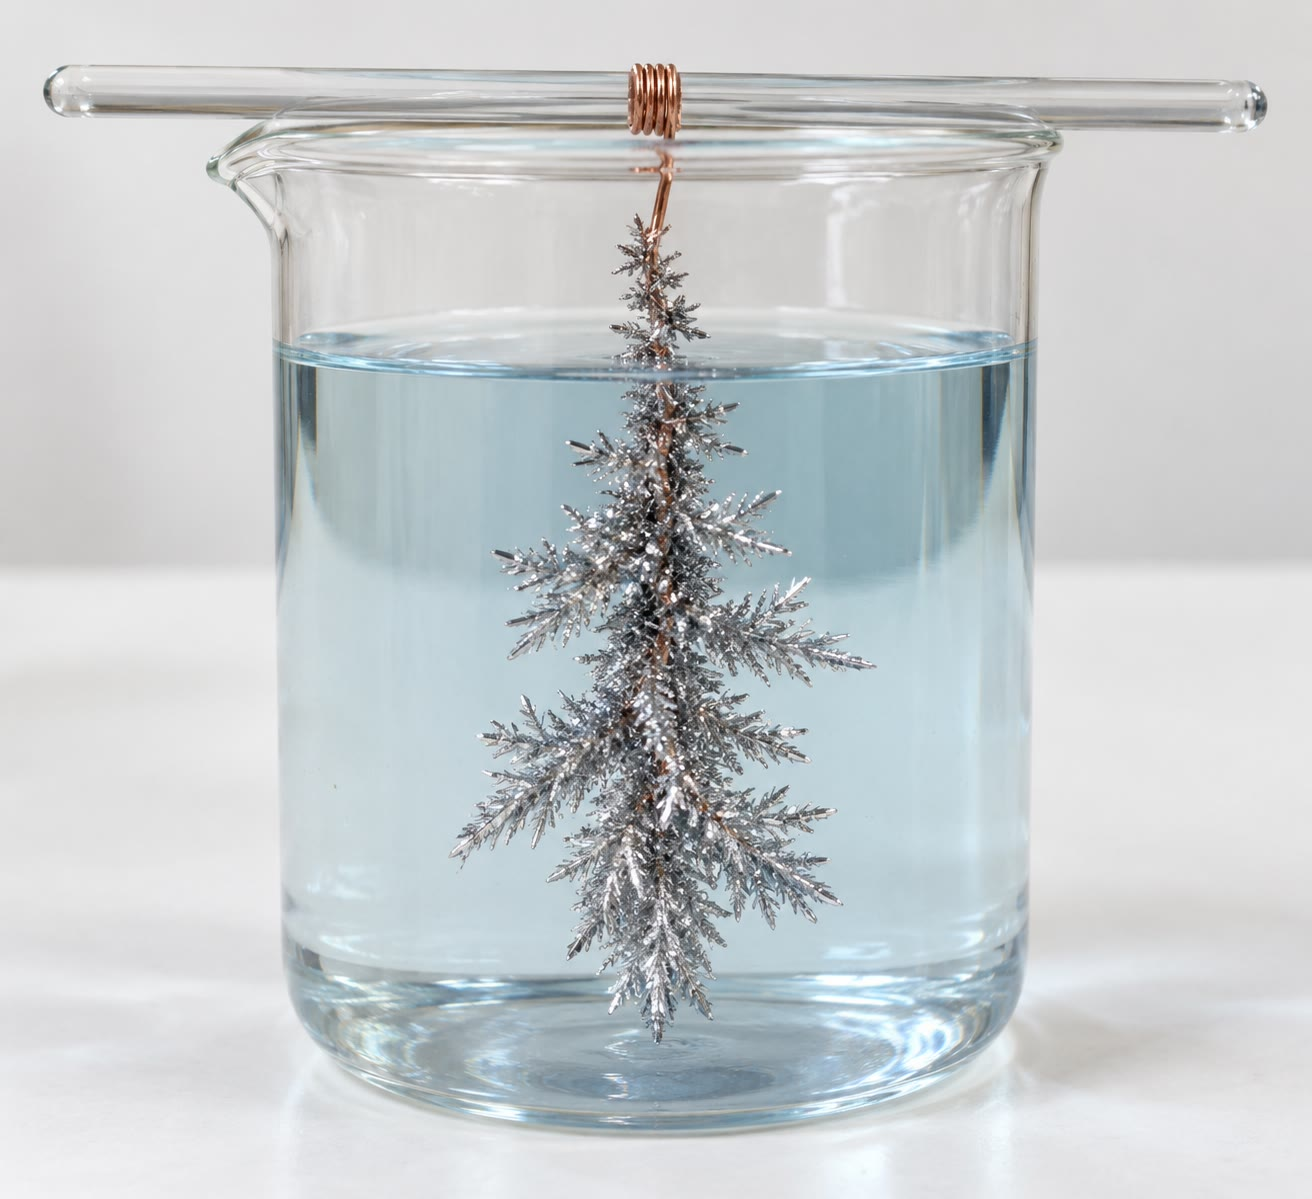
\includegraphics[width=0.5\linewidth]{images/book1/ai/g11-silver-tree.jpg}

{\small Des cristaux d'argent qui poussent sur un fil de cuivre dans une
solution de nitrate d'argent.}
\end{omfigure}

\section{Ajuster les demi-équations}

Beaucoup de couples importants contiennent de l'oxygène et s'écrivent
pour des \omterm{def:g9:acids-bases-ph:acidic}{solutions acides}, où des \omterm{def:g9:ions:ion}{ions} \ce{H+} sont présents. Leurs
\omterm{def:g11:redox:couple}{demi-équations} demandent des \omterm{def:g7:atoms-and-molecules:molecule}{molécules} d'eau et des \omterm{def:g9:ions:ion}{ions} \ce{H+} pour
être ajustées.

\begin{method}[Ajuster une demi-équation en milieu acide]\label{met:g11:redox:balance}
Pour écrire la \omterm{def:g11:redox:couple}{demi-équation} d'un couple Ox/Red en milieu acide~:
\begin{enumerate}
  \item écrire Ox à gauche et Red à droite, et ajuster l'élément qui
        n'est ni O ni H~;
  \item ajuster les \omterm{def:g7:atoms-and-molecules:atom}{atomes} d'oxygène avec des \omterm{def:g7:atoms-and-molecules:molecule}{molécules} d'eau \ce{H2O}~;
  \item ajuster les \omterm{def:g7:atoms-and-molecules:atom}{atomes} d'hydrogène avec des \omterm{def:g9:ions:ion}{ions} \ce{H+}~;
  \item ajuster les charges avec des \omterm{def:g9:inside-the-atom:nucleus}{électrons} \ce{e-}, à gauche~;
  \item vérifier~: même nombre de chaque \omterm{def:g7:atoms-and-molecules:atom}{atome}, même charge totale des
        deux côtés.
\end{enumerate}
\end{method}

\begin{example}[L'ion permanganate]\label{ex:g11:redox:permanganate}
Pour le couple \ce{MnO4^-}/\ce{Mn^{2+}} (du violet foncé au presque
incolore)~: le manganèse est ajusté~; les quatre O de gauche donnent
$\ce{4H2O}$ à droite~; leurs huit H donnent $\ce{8H+}$ à gauche~; la
charge vaut $-1 + 8 = +7$ à gauche, $+2$ à droite, donc on ajoute cinq
\omterm{def:g9:inside-the-atom:nucleus}{électrons} à gauche~:
\[
  \ce{MnO4^-(aq) + 8H+(aq) + 5e- <=> Mn^{2+}(aq) + 4H2O(l)}.
\]
\end{example}

\begin{example}[L'ion dichromate]\label{ex:g11:redox:dichromate}
Pour \ce{Cr2O7^{2-}}/\ce{Cr^{3+}} (de l'orange au vert)~: deux chromes à
droite~; sept O donnent \ce{7H2O}~; quatorze H donnent \ce{14H+}~;
charge $-2 + 14 = +12$ à gauche contre $2 \times 3 = +6$ à droite, donc
six \omterm{def:g9:inside-the-atom:nucleus}{électrons}~:
\[
  \ce{Cr2O7^{2-}(aq) + 14H+(aq) + 6e- <=> 2Cr^{3+}(aq) + 7H2O(l)}.
\]
\end{example}

\begin{method}[Écrire une équation d'oxydoréduction]\label{met:g11:redox:combine}
Pour écrire l'équation de la réaction entre l'\omterm{def:g11:redox:oxidant}{oxydant} Ox$_1$ d'un couple
et le \omterm{def:g11:redox:oxidant}{réducteur} Red$_2$ d'un autre~:
\begin{enumerate}
  \item écrire les deux \omterm{def:g11:redox:couple}{demi-équations}, la première dans le sens de la
        \omterm{def:g11:redox:oxidation}{réduction} (Ox$_1 \to$ Red$_1$), la seconde dans le sens de
        l'\omterm{def:g11:redox:oxidation}{oxydation} (Red$_2 \to$ Ox$_2$)~;
  \item les multiplier par les plus petits nombres qui rendent égaux les
        \omterm{def:g9:inside-the-atom:nucleus}{électrons}~;
  \item les additionner~; les \omterm{def:g9:inside-the-atom:nucleus}{électrons} s'éliminent, de même que
        certains \ce{H+} et \ce{H2O} présents des deux côtés~;
  \item vérifier encore une fois les \omterm{def:g7:atoms-and-molecules:atom}{atomes} et les charges.
\end{enumerate}
\end{method}

\begin{example}[Le permanganate et le fer(II)]\label{ex:g11:redox:mno4-fe}
L'\omterm{def:g9:ions:ion}{ion} permanganate oxyde les \omterm{def:g9:ions:ion}{ions} \ce{Fe^{2+}} en \ce{Fe^{3+}}~:
\[
\begin{array}{l@{\qquad}l}
  \ce{MnO4^- + 8H+ + 5e- -> Mn^{2+} + 4H2O} & \times 1\\
  \ce{Fe^{2+} -> Fe^{3+} + e-} & \times 5\\
  \hline
  \ce{MnO4^- + 8H+ + 5Fe^{2+} -> Mn^{2+} + 5Fe^{3+} + 4H2O} &
\end{array}
\]
Charge à gauche~: $-1 + 8 + 10 = +17$~; à droite~: $2 + 15 = +17$.
Cette réaction sert au chapitre suivant à mesurer une quantité de
fer(II).
\end{example}

\section{Oxydants et réducteurs autour de nous}

\begin{proposition}[Quelques oxydants et réducteurs courants]\label{prop:g11:redox:common}
Les espèces suivantes se rencontrent sans cesse au laboratoire et dans
la vie courante~:
\begin{center}
\small
\begin{tabular}{lll}
\hline
espèce & rôle & \omterm{def:g11:redox:couple}{demi-équation} de son couple \\
\hline
dioxygène \ce{O2} & \omterm{def:g11:redox:oxidant}{oxydant} & \ce{O2 + 4H+ + 4e- <=> 2H2O} \\
dichlore \ce{Cl2} & \omterm{def:g11:redox:oxidant}{oxydant} & \ce{Cl2 + 2e- <=> 2Cl-} \\
hypochlorite \ce{ClO-} (eau de Javel) & \omterm{def:g11:redox:oxidant}{oxydant} & \ce{2ClO- + 4H+ + 2e- <=> Cl2 + 2H2O} \\
peroxyde d'hydrogène \ce{H2O2} & \omterm{def:g11:redox:oxidant}{oxydant} & \ce{H2O2 + 2H+ + 2e- <=> 2H2O} \\
permanganate \ce{MnO4^-} & \omterm{def:g11:redox:oxidant}{oxydant} & \ce{MnO4^- + 8H+ + 5e- <=> Mn^{2+} + 4H2O} \\
métaux \ce{M} (\ce{Fe}, \ce{Zn}, \ce{Al}\dots) & \omterm{def:g11:redox:oxidant}{réducteurs} & \ce{M^{n+} + $n$ e- <=> M} % ce-unbalanced-ok (generic)
\\
iodure \ce{I-} & \omterm{def:g11:redox:oxidant}{réducteur} & \ce{I2 + 2e- <=> 2I-} \\
thiosulfate \ce{S2O3^{2-}} & \omterm{def:g11:redox:oxidant}{réducteur} & \ce{S4O6^{2-} + 2e- <=> 2S2O3^{2-}} \\
acide ascorbique \ce{C6H8O6} (vitamine C) & \omterm{def:g11:redox:oxidant}{réducteur} & \ce{C6H6O6 + 2H+ + 2e- <=> C6H8O6} \\
\hline
\end{tabular}
\end{center}
\end{proposition}

\begin{example}[Le cuivre qui verdit]\label{ex:g11:redox:patina}
Les toits et les statues de cuivre, laissés des dizaines d'années à
l'\omterm{def:g4:air-a-mixture-of-gases:air}{air} libre, prennent lentement une teinte vert pâle. Le dioxygène de
l'\omterm{def:g4:air-a-mixture-of-gases:air}{air} oxyde le cuivre en \omterm{def:g9:ions:ion}{ions} \ce{Cu^{2+}}, qui forment avec l'eau et le
dioxyde de carbone une fine croûte verte, la patine. Contrairement à la
\omterm{def:g9:metals-acids-corrosion:corrosion}{rouille} sur le fer, la patine adhère au \omterm{def:g9:periodic-table-first-look:metal}{métal} et le protège de toute
attaque ultérieure.
\end{example}

\begin{omfigure}
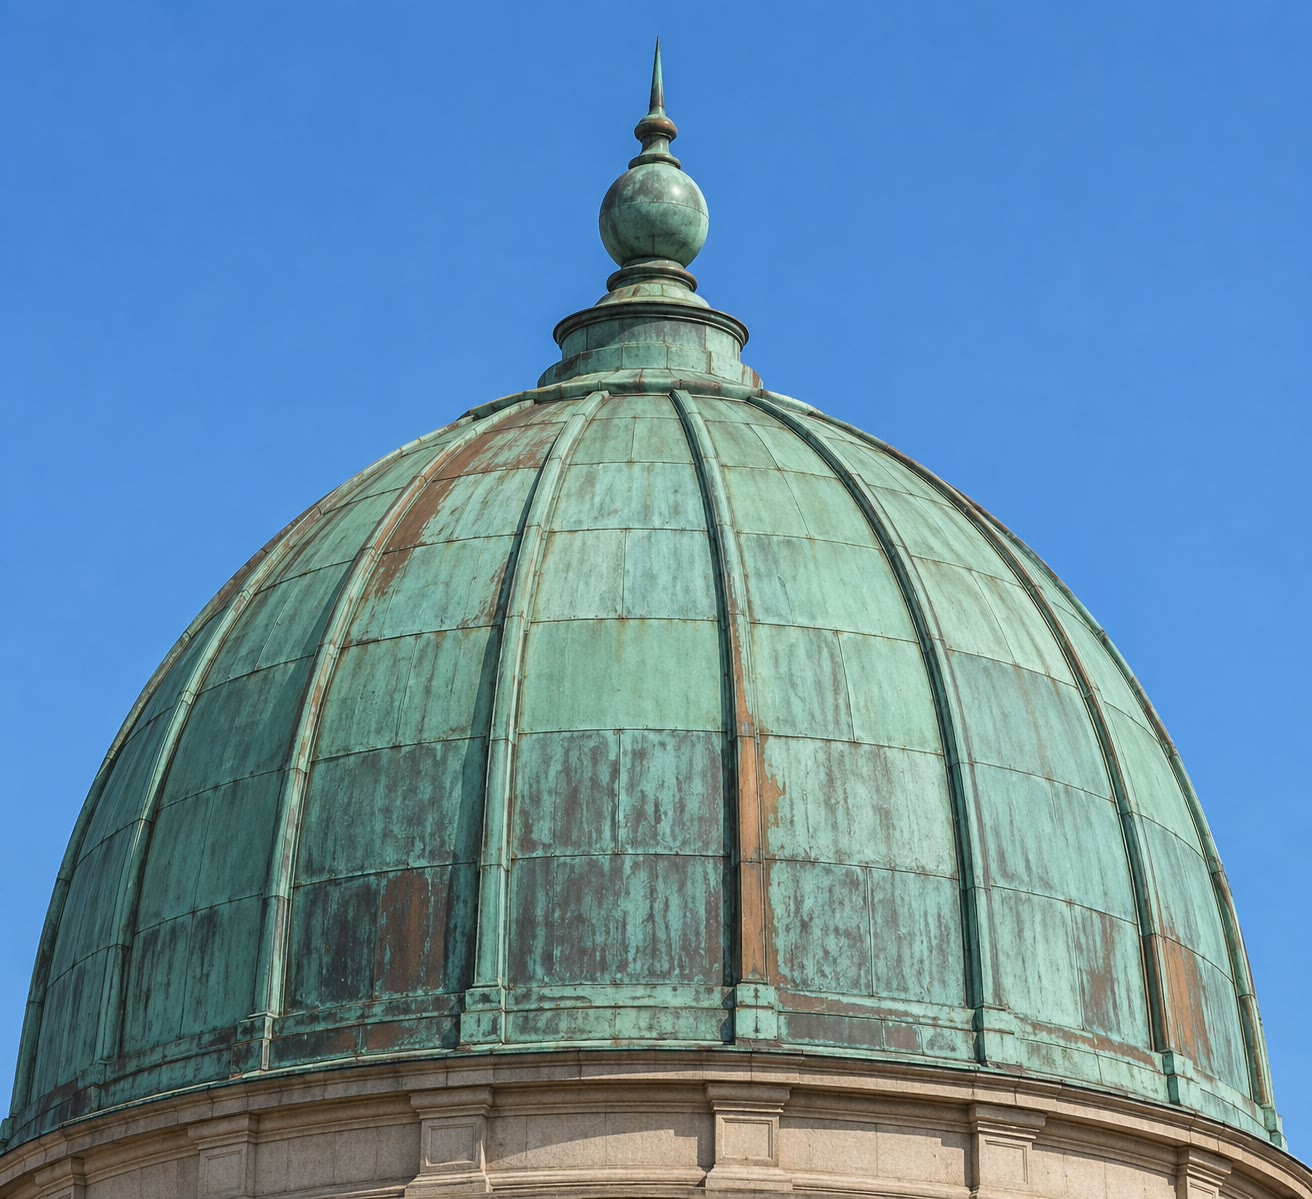
\includegraphics[width=0.48\linewidth]{images/book1/ai/g11-green-roof.jpg}

{\small Un toit de cuivre après des dizaines d'années à l'\omterm{def:g4:air-a-mixture-of-gases:air}{air}~: le
cuivre oxydé forme une patine verte.}
\end{omfigure}

\begin{remark}[Les antioxydants]\label{rem:g11:redox:antioxidant}
Un «~antioxydant~» ajouté aux aliments est un \omterm{def:g11:redox:oxidant}{réducteur} qui est oxydé
par le dioxygène de l'\omterm{def:g4:air-a-mixture-of-gases:air}{air} avant l'aliment. La vitamine C (acide
ascorbique) est le plus courant~: une pomme coupée arrosée de jus de
citron brunit beaucoup plus lentement, parce que la vitamine C du citron
s'oxyde la première.
\end{remark}

\section{Exercices}

\begin{exercise}[$\star$]\label{exo:g11:redox:1}
Définir un \omterm{def:g11:redox:oxidant}{oxydant}, un \omterm{def:g11:redox:oxidant}{réducteur}, une \omterm{def:g11:redox:oxidation}{oxydation} et une \omterm{def:g11:redox:oxidation}{réduction}.
\end{exercise}

\begin{exercise}[$\star$]\label{exo:g11:redox:2}
Pour chaque paire, écrire le \omterm{def:g11:redox:couple}{couple oxydant/réducteur} sous la forme
Ox/Red~: \ce{Fe} et \ce{Fe^{2+}}~; \ce{Ag} et \ce{Ag+}~; \ce{I-} et
\ce{I2}~; \ce{Fe^{2+}} et \ce{Fe^{3+}}.
\end{exercise}

\begin{exercise}[$\star$]\label{exo:g11:redox:3}
Écrire les \omterm{def:g11:redox:couple}{demi-équations} des couples \ce{Ag+}/\ce{Ag},
\ce{Al^{3+}}/\ce{Al}, \ce{Fe^{3+}}/\ce{Fe^{2+}} et \ce{Cl2}/\ce{Cl-}.
\end{exercise}

\begin{exercise}[$\star$]\label{exo:g11:redox:4}
La transformation \ce{Fe -> Fe^{2+} + 2e-} est-elle une \omterm{def:g11:redox:oxidation}{oxydation} ou une
\omterm{def:g11:redox:oxidation}{réduction}~? Le fer joue-t-il le rôle d'\omterm{def:g11:redox:oxidant}{oxydant} ou de \omterm{def:g11:redox:oxidant}{réducteur}~?
\end{exercise}

\begin{exercise}[$\star$]\label{exo:g11:redox:5}
Dans la réaction \ce{Zn + Cu^{2+} -> Zn^{2+} + Cu}, nommer l'espèce
oxydée, l'espèce réduite, l'\omterm{def:g11:redox:oxidant}{oxydant} et le \omterm{def:g11:redox:oxidant}{réducteur}, et donner le nombre
d'\omterm{def:g9:inside-the-atom:nucleus}{électrons} transférés pour chaque \omterm{def:g7:atoms-and-molecules:atom}{atome} de zinc.
\end{exercise}

\begin{exercise}[$\star\star$]\label{exo:g11:redox:6}
Ajuster, en milieu acide, la \omterm{def:g11:redox:couple}{demi-équation} du couple
\ce{H2O2}/\ce{H2O}, en suivant pas à pas la
\cref{met:g11:redox:balance}.
\end{exercise}

\begin{exercise}[$\star\star$]\label{exo:g11:redox:7}
Écrire l'équation de la réaction entre le diiode \ce{I2} et l'\omterm{def:g9:ions:ion}{ion}
thiosulfate \ce{S2O3^{2-}}, qui donne des \omterm{def:g9:ions:ion}{ions} iodure et des \omterm{def:g9:ions:ion}{ions}
tétrathionate \ce{S4O6^{2-}}.
\end{exercise}

\begin{exercise}[$\star\star$]\label{exo:g11:redox:8}
Écrire l'équation de la réaction de l'arbre de Diane à partir de ses
deux \omterm{def:g11:redox:couple}{demi-équations}, et expliquer pourquoi la solution devient bleue.
\end{exercise}

\begin{exercise}[$\star\star$]\label{exo:g11:redox:9}
La vitamine C, \ce{C6H8O6}, réagit avec le diiode \ce{I2}. Écrire
l'équation de la réaction, et dire quelle espèce est le \omterm{def:g11:redox:oxidant}{réducteur}.
\end{exercise}

\begin{exercise}[$\star\star$]\label{exo:g11:redox:10}
L'aluminium réagit avec les \omterm{def:g9:ions:ion}{ions} cuivre(II). Écrire l'équation, et
expliquer pourquoi les \omterm{def:g11:redox:couple}{demi-équations} doivent être multipliées par 2 et
par 3.
\end{exercise}

\begin{exercise}[$\star\star$]\label{exo:g11:redox:11}
Le peroxyde d'hydrogène oxyde les \omterm{def:g9:ions:ion}{ions} fer(II) en \omterm{def:g9:ions:ion}{ions} fer(III) en
milieu acide. Écrire l'équation.
\end{exercise}

\begin{exercise}[$\star\star\star$]\label{exo:g11:redox:12}
Une lame de zinc perd \qty{1.30}{g} dans une solution contenant un excès
d'\omterm{def:g9:ions:ion}{ions} cuivre(II). Quelle masse de cuivre se dépose~? On prendra
$M(\ce{Zn}) = \qty{65.4}{g/mol}$ et $M(\ce{Cu}) = \qty{63.5}{g/mol}$.
\end{exercise}

\begin{exercise}[$\star\star\star$]\label{exo:g11:redox:13}
Écrire l'équation de l'\omterm{def:g11:redox:oxidation}{oxydation} des \omterm{def:g9:ions:ion}{ions} fer(II) par les \omterm{def:g9:ions:ion}{ions}
dichromate en milieu acide. Quelle quantité de \ce{Fe^{2+}} est oxydée
par \qty{0.010}{mol} d'\omterm{def:g9:ions:ion}{ions} dichromate~?
\end{exercise}

\begin{exercise}[$\star\star\star$]\label{exo:g11:redox:14}
L'eau de Javel contient des \omterm{def:g9:ions:ion}{ions} hypochlorite \ce{ClO-} et des \omterm{def:g9:ions:ion}{ions}
chlorure \ce{Cl-}. À l'aide des couples \ce{ClO-}/\ce{Cl2} et
\ce{Cl2}/\ce{Cl-}, écrire l'équation de la réaction qui se produit quand
l'eau de Javel rencontre un acide, et expliquer pourquoi les étiquettes
de l'eau de Javel et des détartrants acides avertissent toutes deux de
ne jamais les \omterm{def:g2:mixing-and-dissolving:mix}{mélanger}.
\end{exercise}

\begin{exercise}[$\star\star\star$]\label{exo:g11:redox:15}
Dans la figure de la surface du zinc, les \omterm{def:g9:inside-the-atom:nucleus}{électrons} traversent le \omterm{def:g9:periodic-table-first-look:metal}{métal},
et non la solution. À l'aide de la
\cref{prop:g11:redox:no-free-electrons}, expliquer pourquoi le cuivre se
dépose sur la lame de zinc elle-même et non ailleurs dans le bécher.
\end{exercise}

\section{Problème~: l'éthylotest}

\begin{problem}[{Problème du week-end --- la chimie d'un éthylotest à
tube~: deux couples, un virage de l'orange au vert, la masse d'éthanol
qu'un tube peut détecter, et la pile à combustible qui l'a remplacé}]
\label{pb:g11:redox:1}
% ledger: ghs:K2Cr2O7, breath:ratio; molar masses from tools/molar_mass.py
% (0.1-rounded weights): K2Cr2O7 294.2, C2H6O 46.0 g/mol
Les premiers éthylotests utilisaient un tube de verre rempli de grains
de silice recouverts de dichromate de potassium orange, \ce{K2Cr2O7}, en
milieu acide. L'éthanol, \ce{CH3CH2OH}, contenu dans l'\omterm{def:g4:air-a-mixture-of-gases:air}{air} expiré que
l'on souffle dans le tube réduit les \omterm{def:g9:ions:ion}{ions} dichromate en \omterm{def:g9:ions:ion}{ions} \ce{Cr^{3+}}
verts et s'oxyde en acide éthanoïque, \ce{CH3COOH}~; la longueur de la
zone verte mesure l'éthanol. On suppose qu'un tube contient
\qty{2.0}{mg} de dichromate de potassium. On utilisera
$M(\ce{K}) = 39.1$, $M(\ce{Cr}) = 52.0$, $M(\ce{O}) = 16.0$,
$M(\ce{C}) = 12.0$, $M(\ce{H}) = \qty{1.0}{g/mol}$, $N_A =
\qty{6.02e23}{mol^{-1}}$ et $e = \qty{1.60e-19}{C}$.

\medskip
\noindent\textbf{Partie I --- Deux couples.}
\begin{enumerate}
  \item Nommer les deux \omterm{def:g11:redox:couple}{couples oxydant/réducteur} mis en jeu, l'\omterm{def:g11:redox:oxidant}{oxydant}
        en premier.
  \item L'éthanol est-il oxydé ou réduit~? Est-il l'\omterm{def:g11:redox:oxidant}{oxydant} ou le
        \omterm{def:g11:redox:oxidant}{réducteur}~?
  \item Écrire la \omterm{def:g11:redox:couple}{demi-équation} du couple \ce{Cr2O7^{2-}}/\ce{Cr^{3+}}
        en milieu acide.
  \item Écrire la \omterm{def:g11:redox:couple}{demi-équation} du couple \ce{CH3COOH}/\ce{CH3CH2OH} en
        milieu acide.
  \item En déduire l'équation de la réaction dans le tube.
\end{enumerate}

\medskip
\noindent\textbf{Partie II --- Ce qu'un tube peut mesurer.}
\begin{enumerate}[resume]
  \item Expliquer le changement de couleur des grains.
  \item Calculer la \omterm{def:g10:the-mole:molar-mass}{masse molaire} du dichromate de potassium.
  \item Calculer la quantité d'\omterm{def:g9:ions:ion}{ions} dichromate dans le tube.
  \item Quelle quantité d'éthanol faut-il pour faire virer au vert tout
        le tube~?
  \item En déduire la plus grande masse d'éthanol qu'un tube peut
        mesurer.
\end{enumerate}

\medskip
\noindent\textbf{Partie III --- De l'haleine au sang.}
Une personne souffle \qty{1.0}{L} d'\omterm{def:g4:air-a-mixture-of-gases:air}{air} dans le tube~; la zone verte
s'allonge proportionnellement à la masse d'éthanol qui l'atteint.
\begin{enumerate}[resume]
  \item L'\omterm{def:g4:air-a-mixture-of-gases:air}{air} expiré contient \qty{0.25}{mg} d'éthanol par litre. Quelle
        fraction du dichromate est utilisée~?
  \item Le tube mesure \qty{10}{cm} de long. Quelle est la longueur de la
        zone verte~?
  \item Les éthylomètres admettent que \qty{2100}{L} d'\omterm{def:g4:air-a-mixture-of-gases:air}{air} expiré
        contiennent autant d'éthanol que \qty{1}{L} de sang. Estimer la
        masse d'éthanol par litre de sang, en grammes.
  \item Pourquoi la zone verte commence-t-elle à l'entrée du tube et
        s'allonge-t-elle vers la sortie, au lieu que tout le tube verdisse
        légèrement~?
  \item Pourquoi un tube ne peut-il servir qu'une fois~?
\end{enumerate}

\medskip
\noindent\textbf{Partie IV --- La pile à \omterm{def:g4:what-a-fire-needs:fuel}{combustible}.}
Le dichromate de potassium porte les pictogrammes
\ghs[0.6cm]{GHS03}\,\ghs[0.6cm]{GHS05}\,\ghs[0.6cm]{GHS06}\,\ghs[0.6cm]{GHS07}\,\ghs[0.6cm]{GHS08}\,\ghs[0.6cm]{GHS09}.
Les appareils modernes utilisent à la place une pile à \omterm{def:g4:what-a-fire-needs:fuel}{combustible}, dans
laquelle l'éthanol de l'\omterm{def:g4:air-a-mixture-of-gases:air}{air} expiré est oxydé par le dioxygène sur une
électrode, et les \omterm{def:g9:inside-the-atom:nucleus}{électrons} libérés circulent dans un fil.
\begin{enumerate}[resume]
  \item Donner deux raisons, lues sur les pictogrammes, pour lesquelles
        on a abandonné les tubes au dichromate.
  \item Écrire l'équation de l'\omterm{def:g11:redox:oxidation}{oxydation} de l'éthanol par le dioxygène,
        à l'aide du couple \ce{O2}/\ce{H2O}.
  \item Combien d'\omterm{def:g9:inside-the-atom:nucleus}{électrons} une \omterm{def:g7:atoms-and-molecules:molecule}{molécule} d'éthanol cède-t-elle quand
        elle est oxydée en acide éthanoïque~?
  \item Pour \qty{0.25}{mg} d'éthanol, calculer la quantité d'éthanol,
        puis le nombre d'\omterm{def:g9:inside-the-atom:nucleus}{électrons} libérés.
  \item En déduire la charge électrique qui traverse la pile à
        \omterm{def:g4:what-a-fire-needs:fuel}{combustible}. Pourquoi cette charge est-elle une bonne mesure de
        l'éthanol de l'haleine~?
\end{enumerate}
\end{problem}
